\chapter{Практическая реализация}
\label{ch:practice}

\section{Авторизация без пароля}

В соответствии с макетом вход в систему реализован без пароля. При
регистрации пользователь вводит e-mail, имя и фамилию
(рисунок~\ref{fig:register}); создаётся учётная запись и генерируется
одноразовый код. Код хранится в базе в виде хеша, действует 10~минут,
используется однократно и блокируется после пяти неверных попыток.

\begin{figure}[h!]
  \centering
  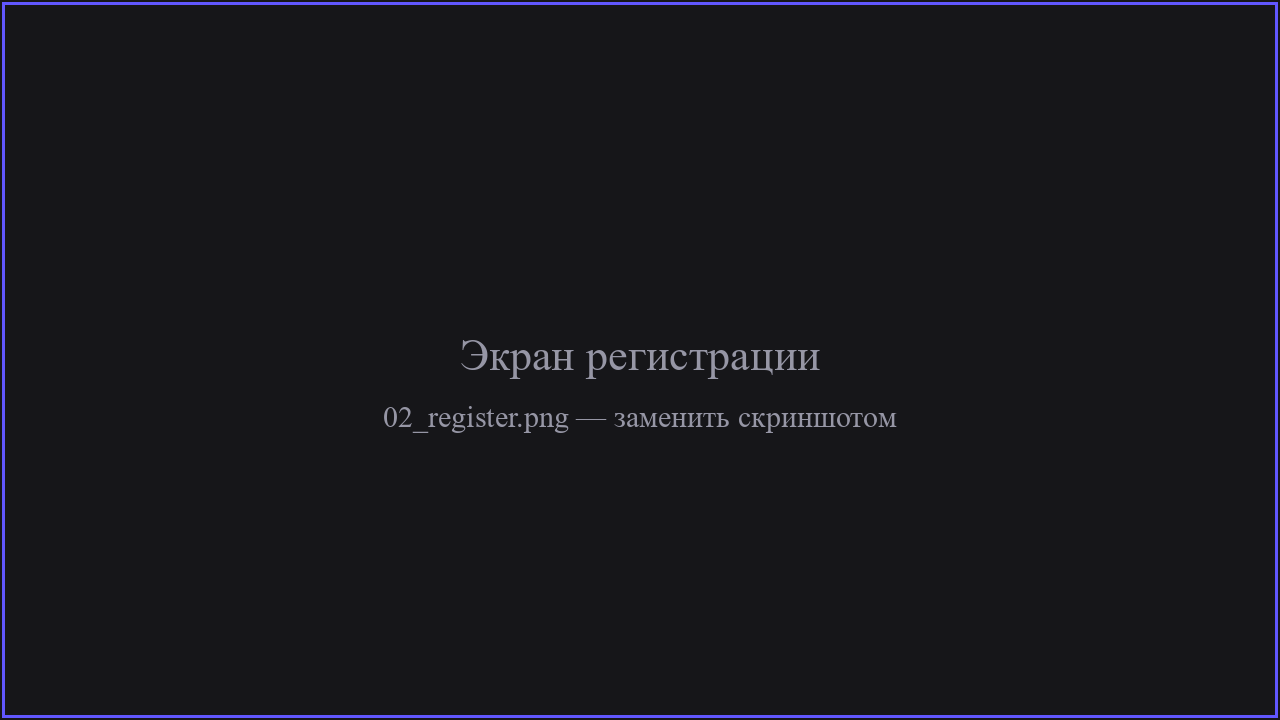
\includegraphics[width=0.55\textwidth]{img/02_register}
  \caption{Экран регистрации}
  \label{fig:register}
\end{figure}

Для входа пользователь указывает e-mail, после чего вводит присланный
код (рисунок~\ref{fig:code}). При локальной разработке письмо выводится
в журнал серверного приложения (рисунок~\ref{fig:emailcode}) --- это
избавляет от необходимости настраивать почтовый сервер для проверки.

\begin{figure}[h!]
  \centering
  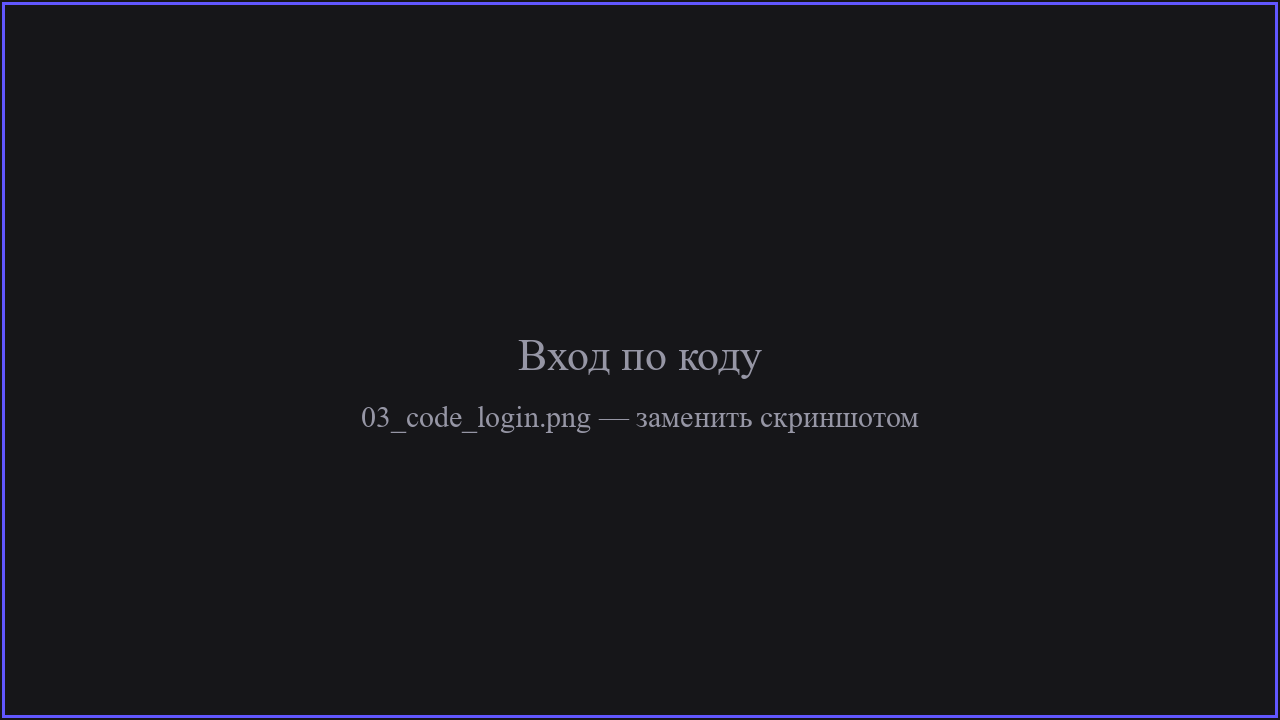
\includegraphics[width=0.55\textwidth]{img/03_code_login}
  \caption{Экран входа по одноразовому коду}
  \label{fig:code}
\end{figure}

\begin{figure}[h!]
  \centering
  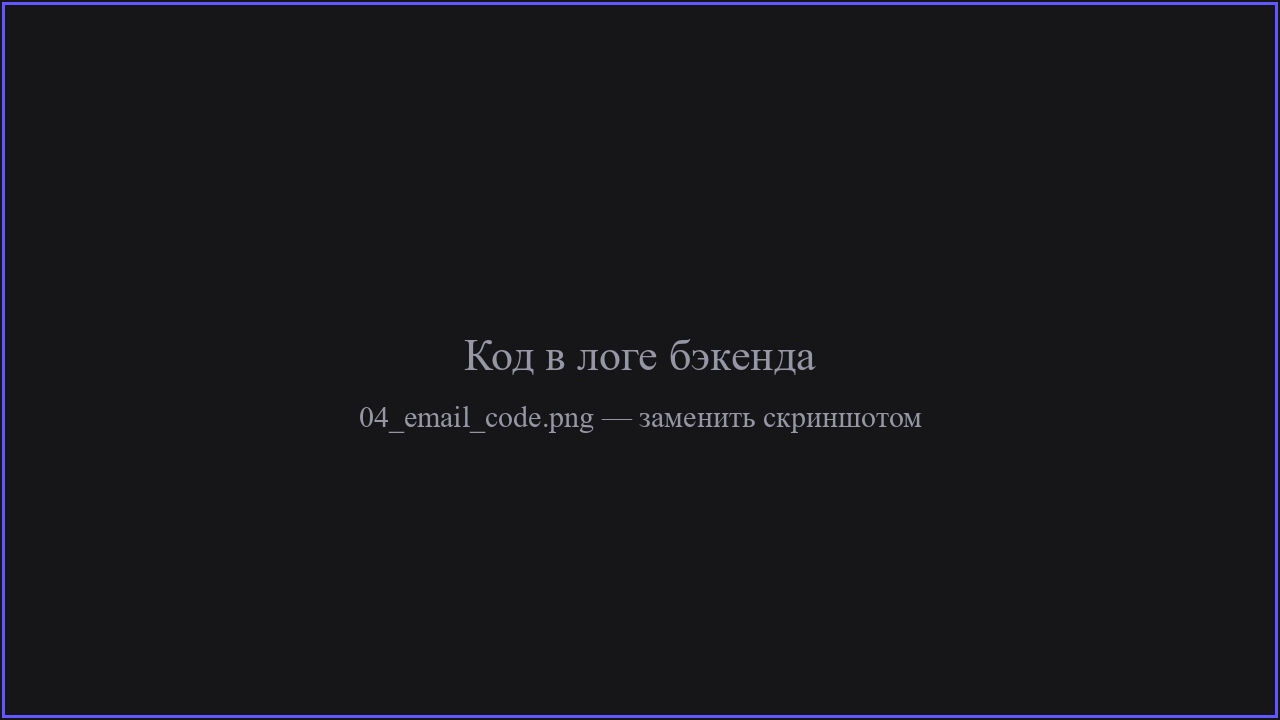
\includegraphics[width=0.9\textwidth]{img/04_email_code}
  \caption{Одноразовый код в журнале серверного приложения}
  \label{fig:emailcode}
\end{figure}

После проверки кода сервер выпускает пару JWT-токенов. Access-токен
хранится в памяти клиентского приложения, refresh-токен --- в
\texttt{localStorage}; при ответе сервера <<401\,>> клиент один раз
автоматически обновляет access-токен и повторяет запрос.

\section{Загрузка и потоковая отдача видео}

Загрузка видео выполняется на отдельной странице
(рисунок~\ref{fig:upload}): пользователь указывает название, описание,
выбирает файл и, при желании, превью. Файл передаётся методом
\texttt{multipart/form-data}; на сервере определяются его размер и
длительность (через \texttt{ffprobe}).

\begin{figure}[h!]
  \centering
  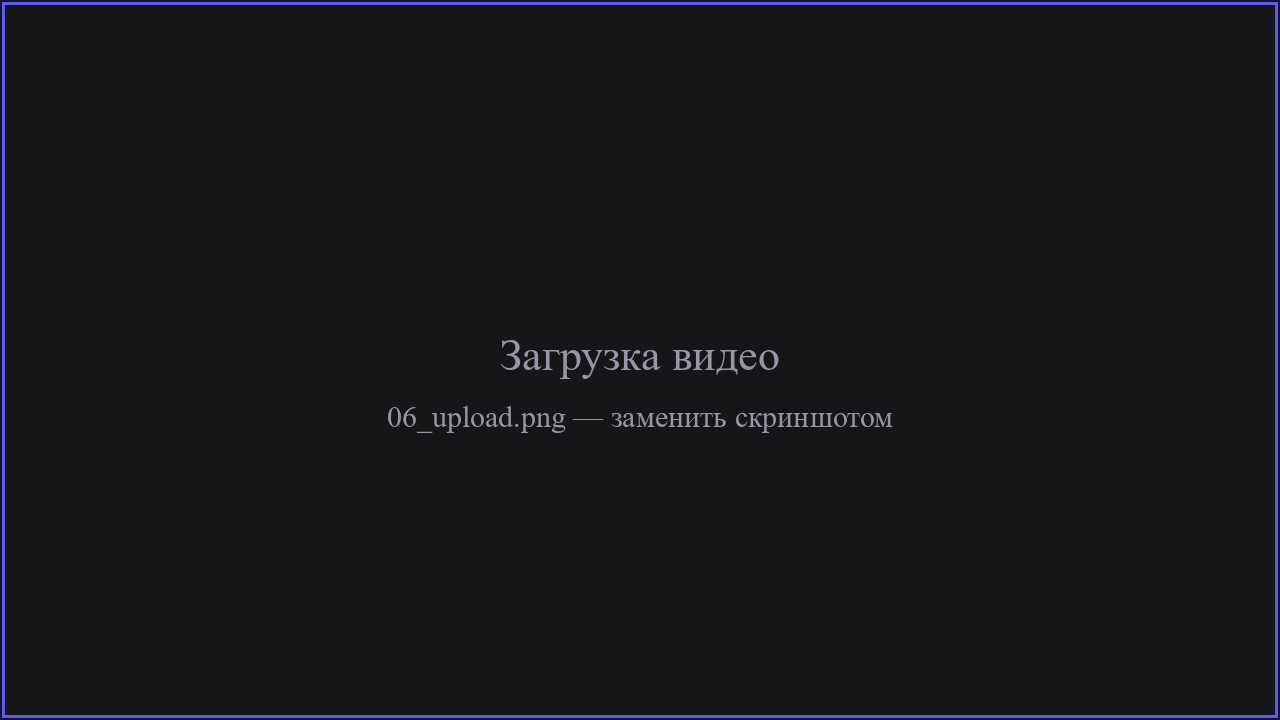
\includegraphics[width=0.6\textwidth]{img/06_upload}
  \caption{Страница загрузки видео}
  \label{fig:upload}
\end{figure}

Потоковая отдача реализована с поддержкой HTTP-заголовка \texttt{Range}:
браузерный плеер при перемотке запрашивает не весь файл, а нужный
фрагмент. Сервер разбирает заголовок и отвечает кодом
<<206~Partial~Content>>, передавая запрошенный диапазон байтов. Функция
отдачи вынесена в приложение \texttt{common} и переиспользуется.

\section{Лента, просмотр и профиль}

Главная страница показывает ленту опубликованных видео с постраничной
подгрузкой (рисунок~\ref{fig:feed}). Страница просмотра содержит плеер,
сведения о ролике и кнопку <<\,Смотреть вместе\,>>, создающую комнату.

\begin{figure}[h!]
  \centering
  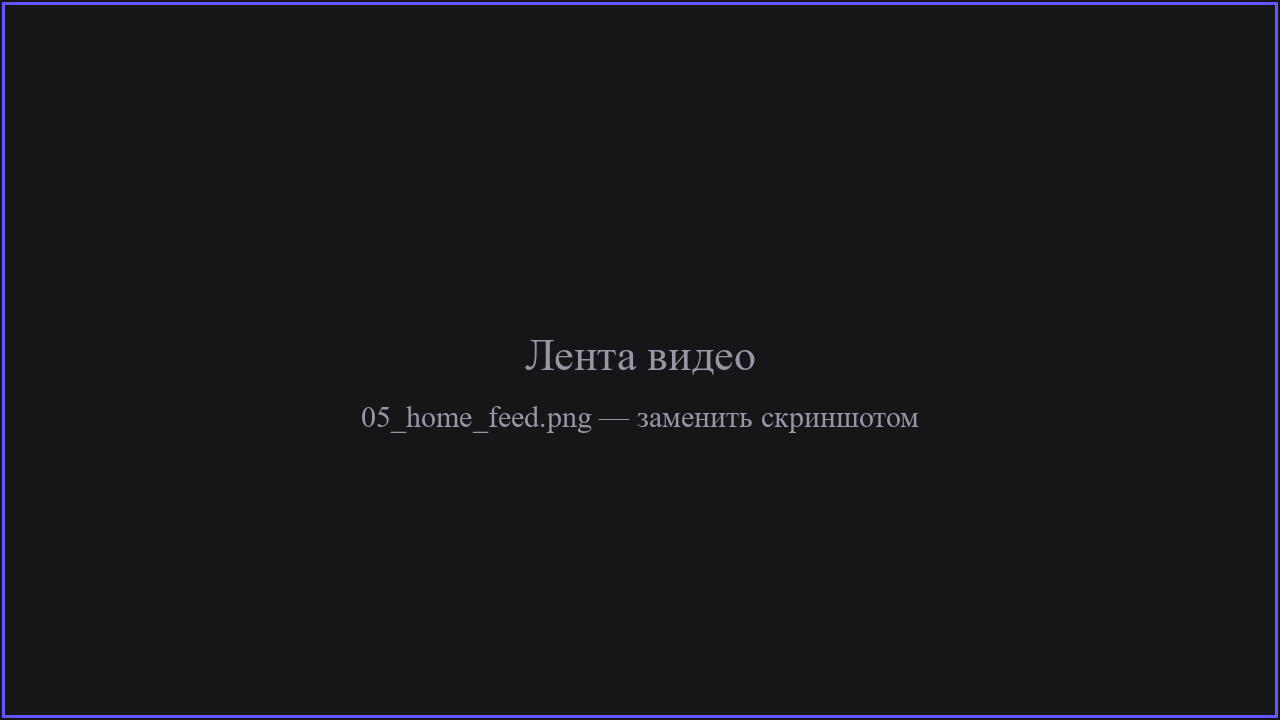
\includegraphics[width=0.9\textwidth]{img/05_home_feed}
  \caption{Лента видео}
  \label{fig:feed}
\end{figure}

\begin{figure}[h!]
  \centering
  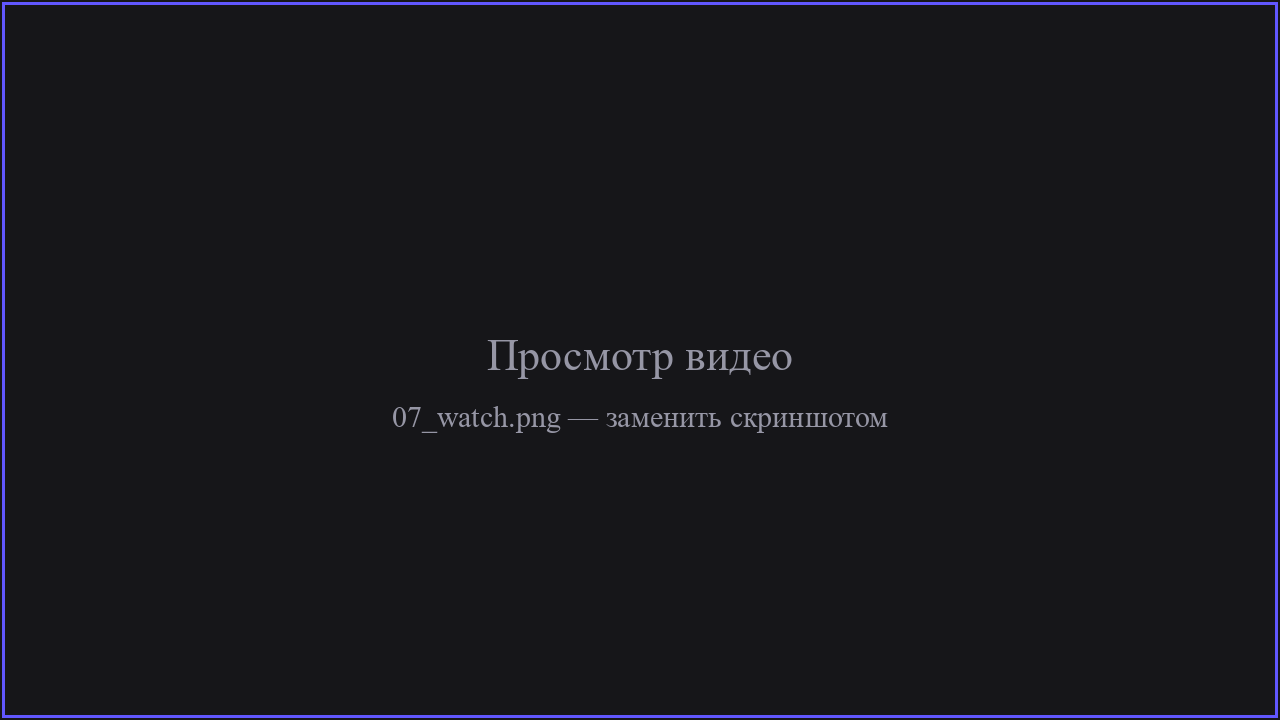
\includegraphics[width=0.9\textwidth]{img/07_watch}
  \caption{Страница одиночного просмотра видео}
  \label{fig:watch}
\end{figure}

На странице профиля пользователь видит свои видео, может их удалять и
редактировать <<\,имя в чате\,>> (рисунок~\ref{fig:profile}).

\begin{figure}[h!]
  \centering
  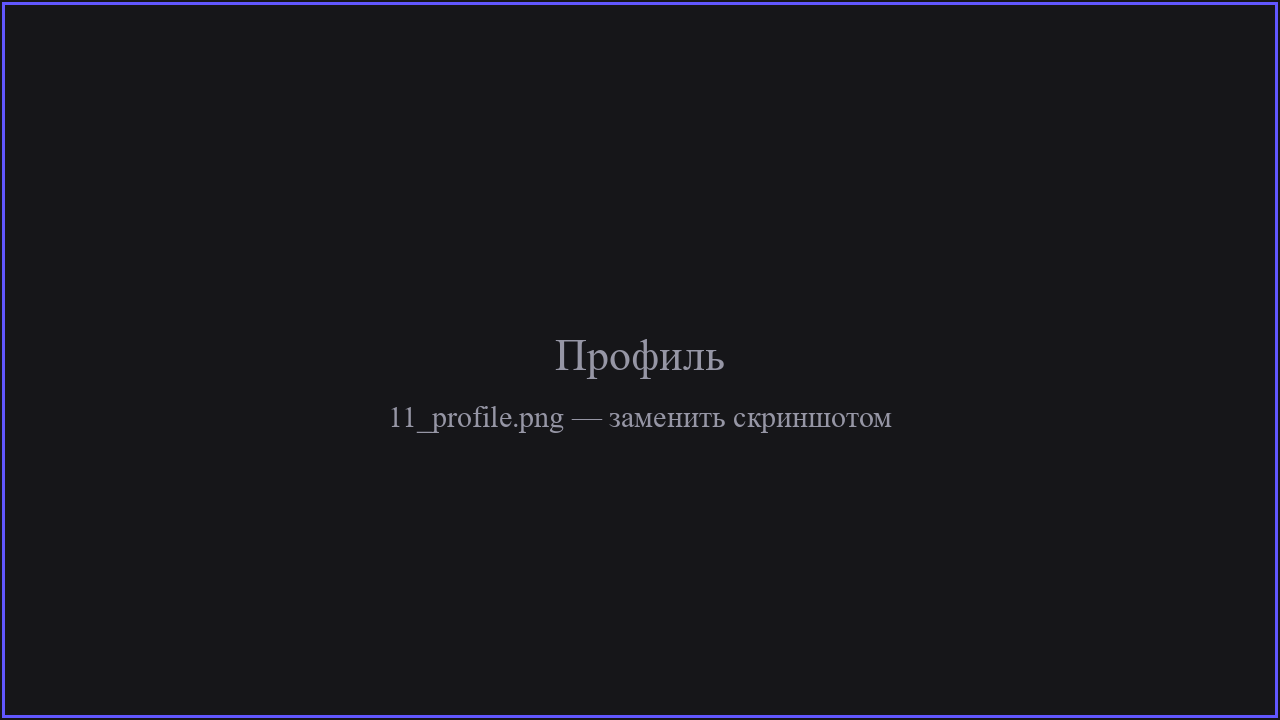
\includegraphics[width=0.9\textwidth]{img/11_profile}
  \caption{Профиль пользователя и управление своими видео}
  \label{fig:profile}
\end{figure}

\section{Комнаты и синхронизация воспроизведения}

Комната совместного просмотра --- сигнатурная функция платформы. Её
страница повторяет макет Figma: слева плеер, справа панель с чатом и
вкладкой вопросов (рисунок~\ref{fig:roomchat}).

\begin{figure}[h!]
  \centering
  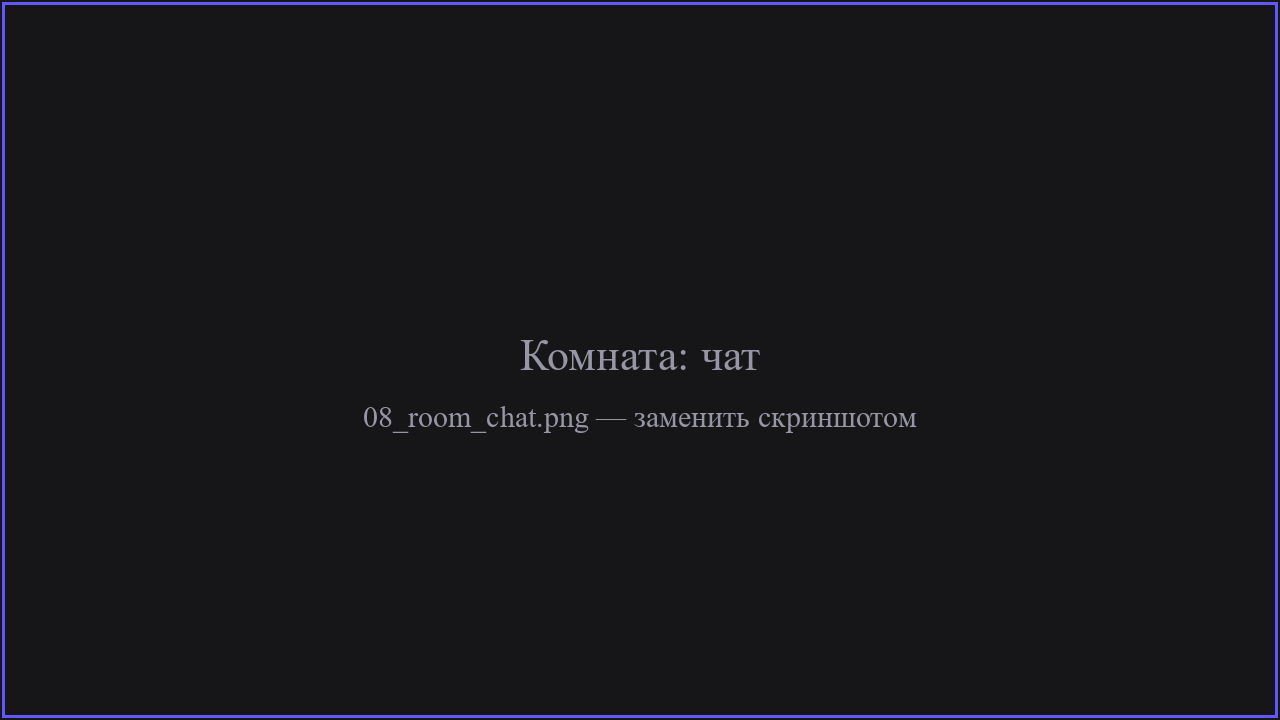
\includegraphics[width=0.95\textwidth]{img/08_room_chat}
  \caption{Комната просмотра: плеер и панель чата с лайками}
  \label{fig:roomchat}
\end{figure}

Синхронизацию обеспечивает WebSocket-консьюмер на стороне сервера и хук
синхронизации на стороне клиента. Команды ведущего изменяют состояние
комнаты в базе и рассылаются всем участникам. Плеер зрителя применяет
полученное состояние, а затем каждые три секунды сверяет позицию:
расхождение более секунды устраняется перемоткой, меньшее --- плавным
изменением скорости. Управление плеером доступно только ведущему, у
зрителя оно скрыто. На рисунке~\ref{fig:roomsync} показаны два окна
браузера: действие ведущего отражается в окне зрителя.

\begin{figure}[h!]
  \centering
  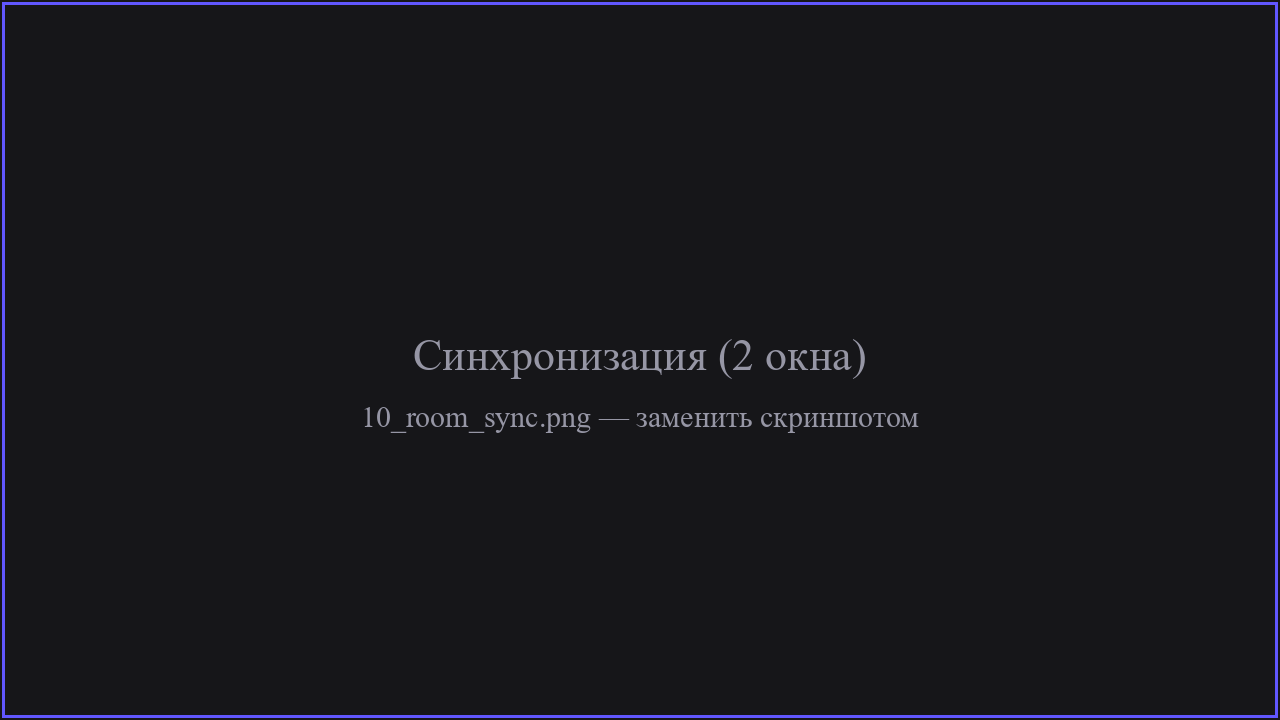
\includegraphics[width=0.95\textwidth]{img/10_room_sync}
  \caption{Синхронизация: ведущий управляет, зритель повторяет}
  \label{fig:roomsync}
\end{figure}

\section{Живой чат и вкладка <<Вопрос/ответ>>}

Боковая панель комнаты содержит две вкладки. На вкладке
<<\,Чат\,>> участники обмениваются сообщениями и ставят лайки ---
сообщение оформлено карточкой из дизайн-системы макета. На вкладке
<<\,Вопрос\,/\,ответ\,>> зрители задают вопросы, отвечают на них и
голосуют (рисунок~\ref{fig:roomqa}). Все события чата идут по тому же
WebSocket-соединению, что и синхронизация; гость может читать чат, но не
писать в него.

\begin{figure}[h!]
  \centering
  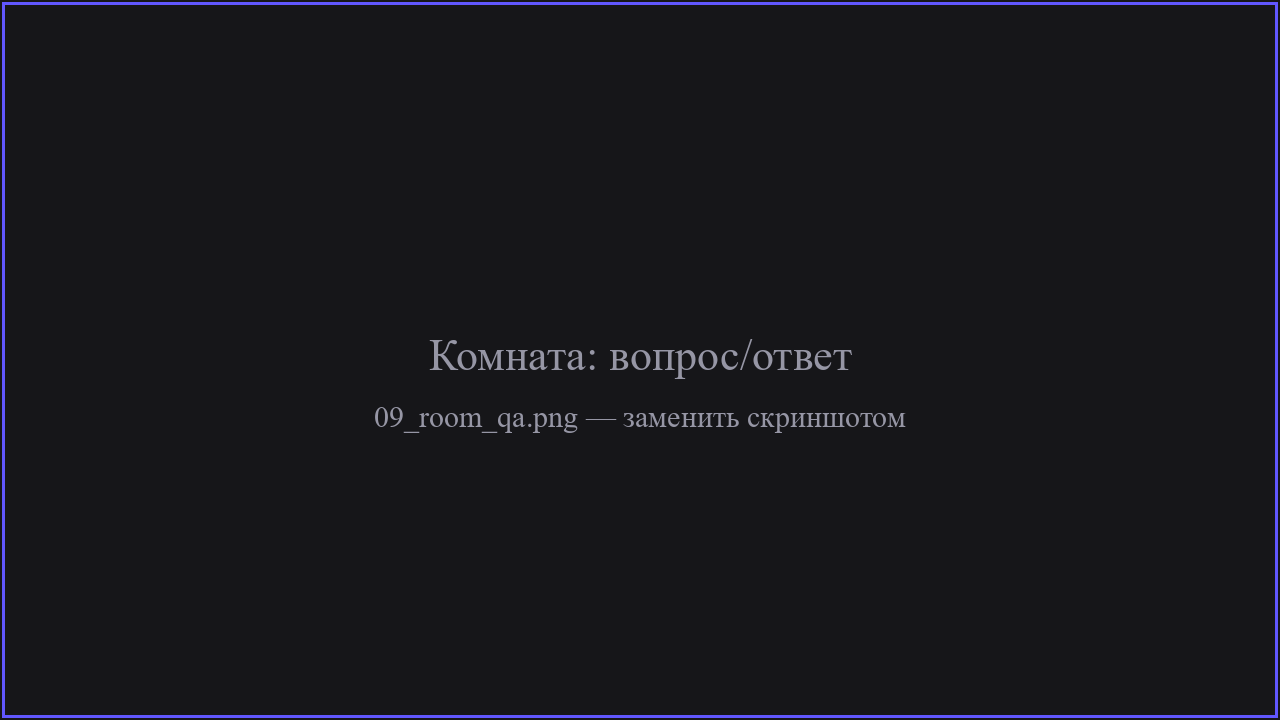
\includegraphics[width=0.95\textwidth]{img/09_room_qa}
  \caption{Вкладка <<Вопрос/ответ>> в комнате просмотра}
  \label{fig:roomqa}
\end{figure}

\section{Клиентское приложение и дизайн-система}

Клиентское приложение собрано на React с маршрутизацией React~Router.
Компоненты дизайн-системы (поле ввода, кнопка, карточка сообщения,
вкладки) перенесены из макета Figma и собраны в отдельный каталог. Все
цвета, отступы и скругления заданы CSS-переменными --- это позволило
перекрасить интерфейс под тёмную тему, не трогая разметку компонентов.
Вёрстка адаптивная: на узких экранах сетка ленты сворачивается в одну
колонку, а панель комнаты переносится под плеер
(рисунок~\ref{fig:mobile}).

\begin{figure}[h!]
  \centering
  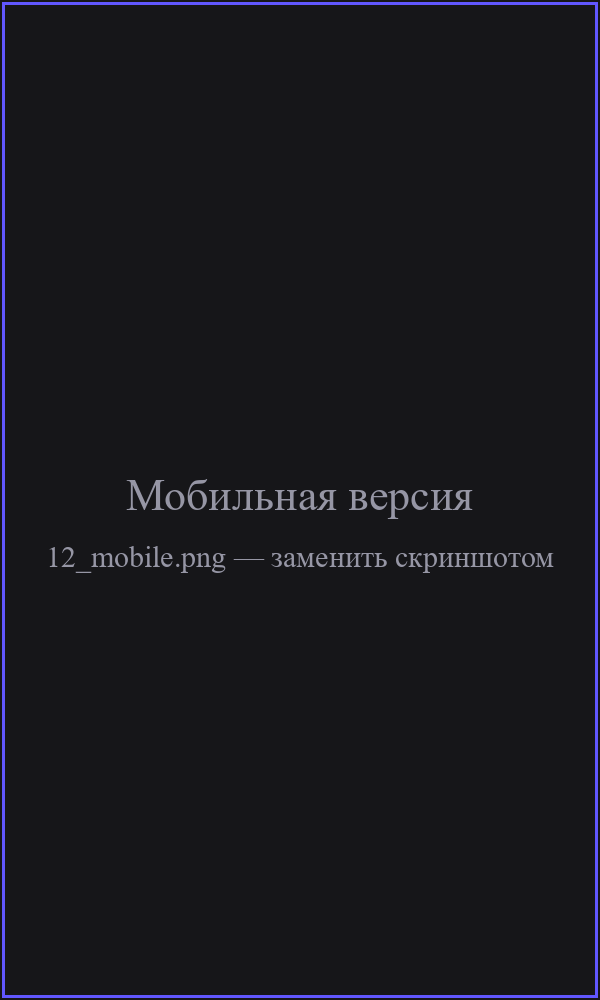
\includegraphics[width=0.4\textwidth]{img/12_mobile}
  \caption{Адаптивная вёрстка на мобильном экране}
  \label{fig:mobile}
\end{figure}

\section{Тестирование}

Серверная часть покрыта тестами \texttt{pytest}: проверяются
авторизация (выдача и проверка кода, блокировка после неверных попыток),
загрузка видео и Range-стриминг, чистая функция расчёта позиции
воспроизведения, а также WebSocket-консьюмер комнаты --- подключение,
синхронизация, чат и запрет управления для гостя
(рисунок~\ref{fig:pytest}).

\begin{figure}[h!]
  \centering
  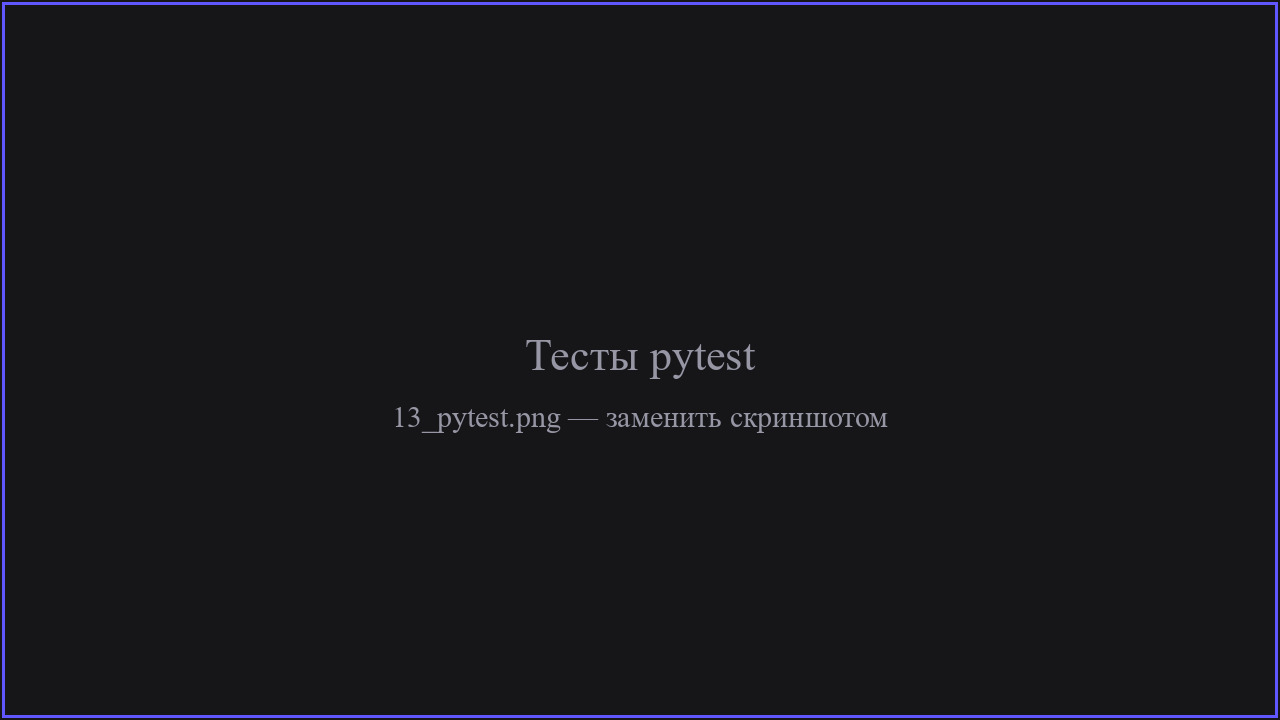
\includegraphics[width=0.9\textwidth]{img/13_pytest}
  \caption{Прогон тестов серверной части (pytest)}
  \label{fig:pytest}
\end{figure}

Клиентская часть покрыта тестами \texttt{Vitest}: проверяются
компоненты дизайн-системы, разбор ответов об ошибках и логика коррекции
рассинхрона плеера (рисунок~\ref{fig:vitest}).

\begin{figure}[h!]
  \centering
  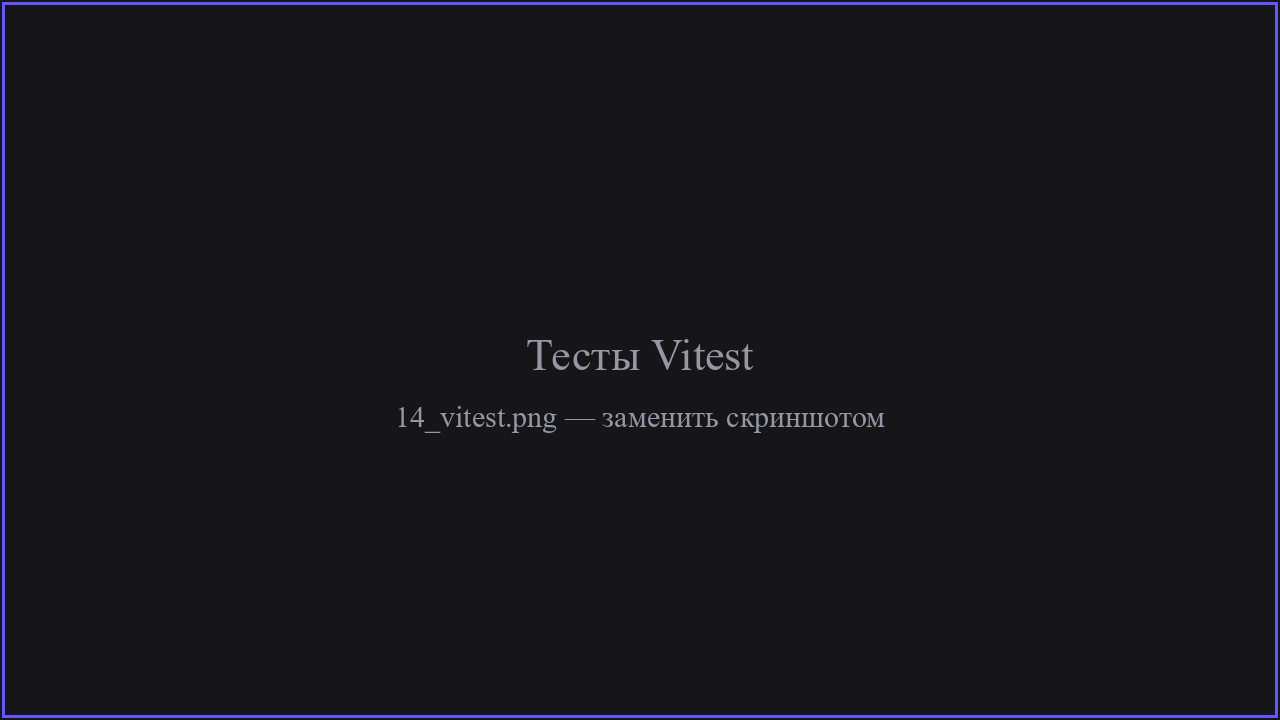
\includegraphics[width=0.9\textwidth]{img/14_vitest}
  \caption{Прогон тестов клиентской части (Vitest)}
  \label{fig:vitest}
\end{figure}

\section{Развёртывание на сервере}

Платформа развёрнута на собственном сервере скриптом \texttt{deploy.sh}:
он поднимает контейнеры базы данных, Redis, серверной и клиентской
частей и подключает поддомен к Caddy (рисунок~\ref{fig:docker}). Доступ
к сайту идёт по защищённому протоколу HTTPS с сертификатом Let's~Encrypt
(рисунок~\ref{fig:https}).

\begin{figure}[h!]
  \centering
  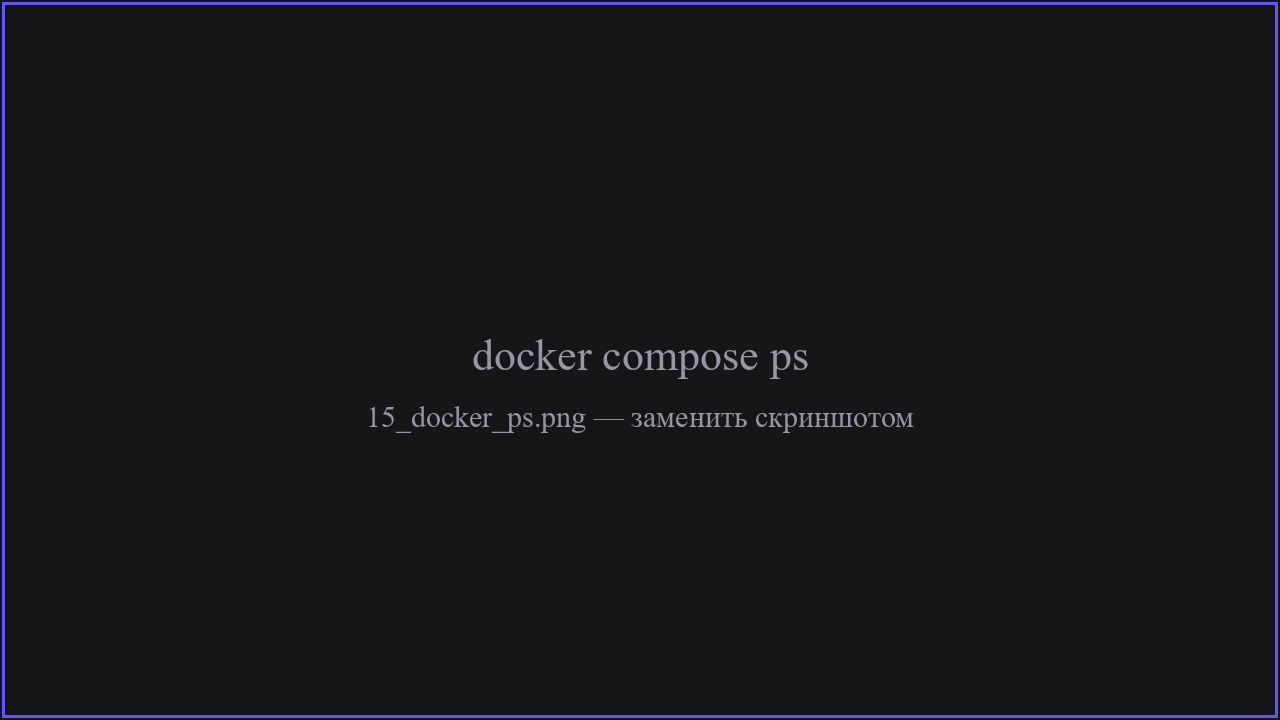
\includegraphics[width=0.9\textwidth]{img/15_docker_ps}
  \caption{Контейнеры blxck.hub, запущенные на сервере}
  \label{fig:docker}
\end{figure}

\begin{figure}[h!]
  \centering
  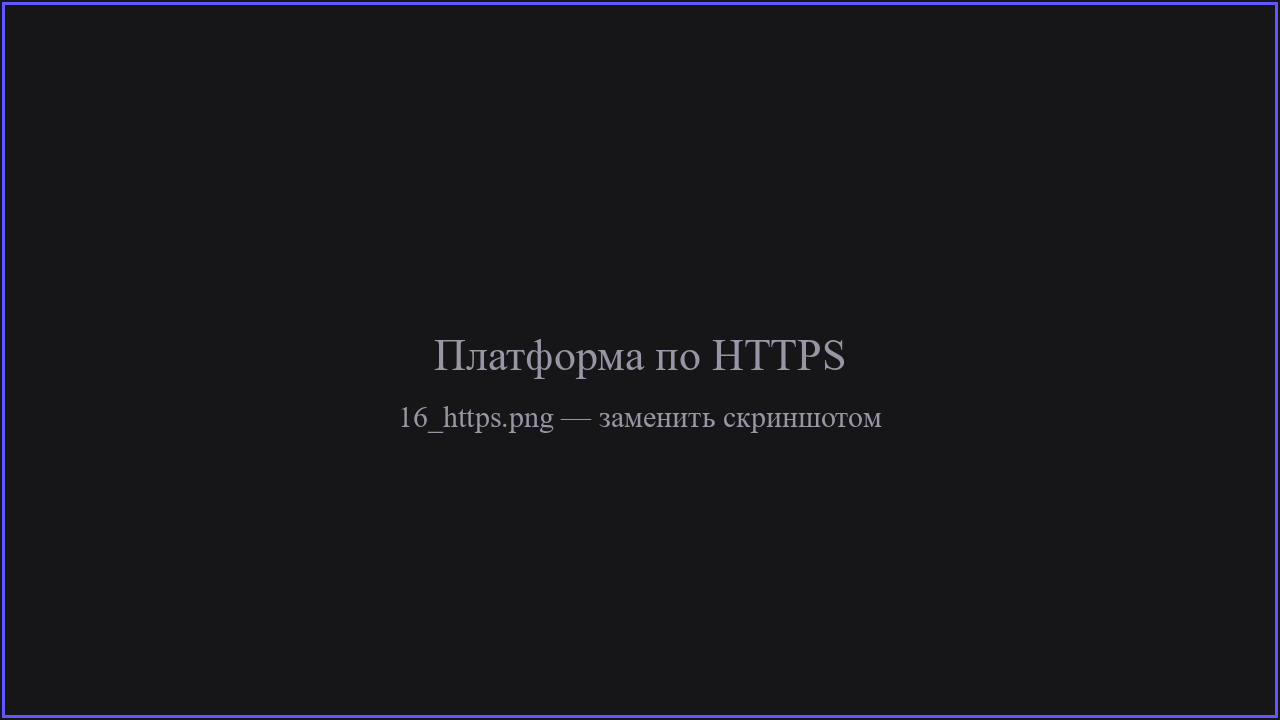
\includegraphics[width=0.9\textwidth]{img/16_https}
  \caption{Платформа доступна по HTTPS}
  \label{fig:https}
\end{figure}

\section{Трудности и пути их решения}

В ходе разработки возникли следующие трудности.

\textbf{Авторизация по WebSocket.} Браузерный WebSocket-API не позволяет
задавать HTTP-заголовок \texttt{Authorization}, поэтому стандартный
способ передачи JWT не работает. Решение --- передавать access-токен
параметром строки запроса, а на сервере разбирать его в промежуточном
слое и подставлять пользователя в сессию соединения.

\textbf{Настройка коррекции рассинхрона.} Жёсткая перемотка плеера
зрителя при каждом расхождении приводила к рывкам изображения. Решение
--- ввести два порога: малый рассинхрон устраняется плавным изменением
скорости воспроизведения, и только значительный --- перемоткой. Логика
вынесена в чистую функцию и покрыта тестами.

\textbf{Автозапуск видео у зрителя.} Браузеры блокируют автоматическое
воспроизведение видео со звуком без действия пользователя, из-за чего
плеер зрителя не запускался. Решение --- показывать поверх плеера
кнопку <<\,Присоединиться к просмотру\,>>: нажатие является нужным
жестом и одновременно запрашивает у сервера актуальное состояние.

\textbf{Отдача больших видеофайлов.} Передача видео целиком на каждый
запрос не позволяла перематывать ролик и нагружала сервер. Решение ---
реализовать поддержку HTTP-заголовка \texttt{Range} с ответом
<<206~Partial~Content>>; статические файлы в продакшене отдаёт nginx.

\textbf{Поле флага в multipart-форме.} При загрузке видео без явного
флага публичности сериализатор трактовал отсутствующее булево поле как
<<\,ложь\,>>, и ролик не попадал в ленту. Решение --- разбирать признак
публичности отдельно во вьюхе, считая отсутствие значения согласием.

\textbf{Единая конфигурация для двух окружений.} Локальная разработка и
продакшен требуют разных баз данных и слоёв каналов. Решение ---
управлять конфигурацией через переменные окружения: без них приложение
использует SQLite и слой каналов в памяти, с ними --- PostgreSQL и
Redis.

\endinput
